\chapter{\babDua}
Membuat desain sebuah perangkat ic membutuhkan proses yang panjang dan sumberdaya manusia yang banyak, serta tingkat ketelitian yang tinggi. Oleh karenanya di butuhkan biaya yang tidak kecil dan waktu yang cukup lama hanya untuk membuat sebuah desain IC. Dengan kerumitan yang tinggi serta waktu yang lama dalam setiap prosesnya kadang pihak yang tak bertanggung jawab melakukan kecurangna dengan mecuri desain untuk memotong waktu dan biaya yang di butuhkan utuk produksi. sehingga menjadi masalah dalam dunia permanufakturan ic.

\section{Large Scale Integration}
\textit{Large Scale Integration} atau disingkat LSI merupakan teknologi desain IC dengan kepadatan gate sekitar xx gate. pada awalnya blablabal...

\subsection{Arus Pengembangan LSI}
\todo{isi perkembangan LSI sesua renesas web}

\subsection{Kemungkinan Serangan Desain LSI}
Terdapat banyak kemungkinan serangan dalam proses manufakturing desain LSI. Berikut beberapa contoh serangan terhadap LSI desain.

\begin{figure}
	\centering
	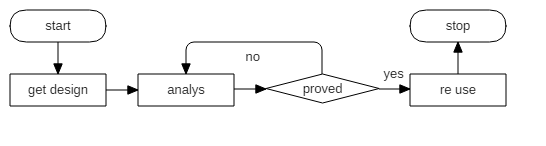
\includegraphics[width=1.05\textwidth]
	{diagrams/untrustSource.png}
	\caption{Clonning/Sumber Tidak Terpercaya}
	\label{fig:untrustsource}
\end{figure}

Dalam segi ini serangan dilakukan dengan cara mencuri langsung desain yang sudah siap di fabrikasi serta uji coba kebenaran. Bila pencuri mendapatkan desain yang telah di uji coba, maka pencuri tinggal langsung memperbanyak desain yang telah di curi.

\begin{figure}
	\centering
	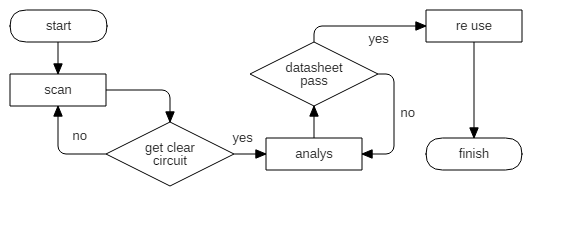
\includegraphics[width=1.05\textwidth]
	{diagrams/reverseEngineering.png}
	\caption{RE (Reverse Engineering)}
	\label{fig:reverseengineering}
\end{figure}

Untuk serangan jenis ini, pencuri sudah pendapatkan produk dari pasar yang telah teruji, pencuri tinggal melakukan scan rangkaian kemudian mengujinya dengan datasheet. Apabila hasil scan desain produk di dapati rangkaian yang konkrit/jelas dan rangkaian tersebut telah teruji sesuai datasheet. Maka pencuri tinggal melakukan fabrikasi.

\subsection{Mengatasi Serangan terhadap Desain LSI}
\todo{jelasin dari buku dan paper gimana cara mengatasinya}

\section{Teknik Proteksi}
Dari berbagai teknik yang telah digunakan, penulis melakukan penggabungan 2 teknik pengamanan dalam sebuah desain IC. Dalam penelitian ini dilakukan penggabungan 2 teknik agar cakupan wilayah keamanan sebuah IC semakin luas. Berikut teknik yang digabungkan dalam penelitian kali ini.

\subsection{DSP (Digital Signal Processing)}
DSP merupakan teknik pengolahan sinyal untuk sinyal digital.

\subsection{Polimorphisme}
Polimorphisme merupakan teknik pengecoh yang di gunakan dalam perlindungan desain IC. 

\section{Peralatan dan Teknologi}
Dalam penelitian kali ini dibutuhkan beberapa peralatan dan standard teknologi untuk mengembangkan teknik perlindungan intelektual properti. Sebagai penunjang dalam pembuatan perlindungan, penulis menggunakan tools dan teknologi yang umum digunakan dalam proses pengembangan desain LSI.

\subsection{Verilog HDL}
Verilog HDL merupakan bahasa pendeskripsi hardware yang di rancang untuk mendeskripsikan suatu rancangan perangkat keras pada gate-lavel dalam bentuk bahasa manusia *walaupun enggak begitu manusiawi

\subsection{YOSYS}
YOSYS adalaha...

\subsection{FPGA Elbert V2 Board}
FPGA merupakan kepanjangan dari Field Programmable Gate Array adalah perangkat keras yang biasa digunakan dalam proses manufakturing IC. FPGA digunakan untuk mensimulasikan draft rancangan IC yang siap untuk di test yang apabila telah lolos test akan di lanjutkan ke tahap layout. FPGA hanya digunakan apabila rancangan membutuhkan input dari perangkat lain atau program kernel.

\section{Target IP Core}
Watermark adalah rangkaian yang tidak dapat berdiri sendiri pada implementasinya walaupun dalam pengembangannya bisa di lakukan mandiri. Watermark dalam bentuk data signature.

\subsection{ALU (Aritmatic Logic Unit)}
Aritmatik Logic Unit atau dapat di singkat sebagai ALU merupakan salah satu komponen utama dalam prosesor. ALU berfungsi sebagai Unit yang melakukan kalkulasi logika artimatika.
